\begin{frame}{Opbevaring af våben og ammunition § 24}

\vspace{1em}

\begin{columns}[c] % c = center vertically

\column{0.05\textwidth} % Venstre margin (kan fjernes eller justeres)



\column{0.7\textwidth} % Midten: Bullets

\small

\raggedright



\begin{itemize}

\itemsep0.6em % Justér afstand mellem bullets

\item Våben og ammunition skal opbevares forsvarligt og \textbf{utilgængeligt} for uvedkommende.

\item Skabe under \textbf{1.000 kg} skal være fastboltet til gulv/væg.

\item Nøgler til skabet skal opbevares separat og utilgængeligt.

\item Der sondres mellem to typer af våbenskabe, som styres af antallet af våben, der skal opbevares.

\item Max 25 regulære våben, hvor max 10 våben må være særligt farlige våben \textbf{kræver} (min. EN 1143-1 \textbf{Grade 0}).

\item Flere end 25 regulære våben og/eller 10 særligt farlige våben \textbf{kræver} (min. EN 1143-1 \textbf{Grade 1}).

\item Ammunition må opbevares ved siden af, men ikke i våbnet.

\end{itemize}



\column{0.25\textwidth} % Højre: Ikon (størrelsen tilpasses her)

\centering

\vspace{0pt} % hjælper med vertikal centring i nogle temaer

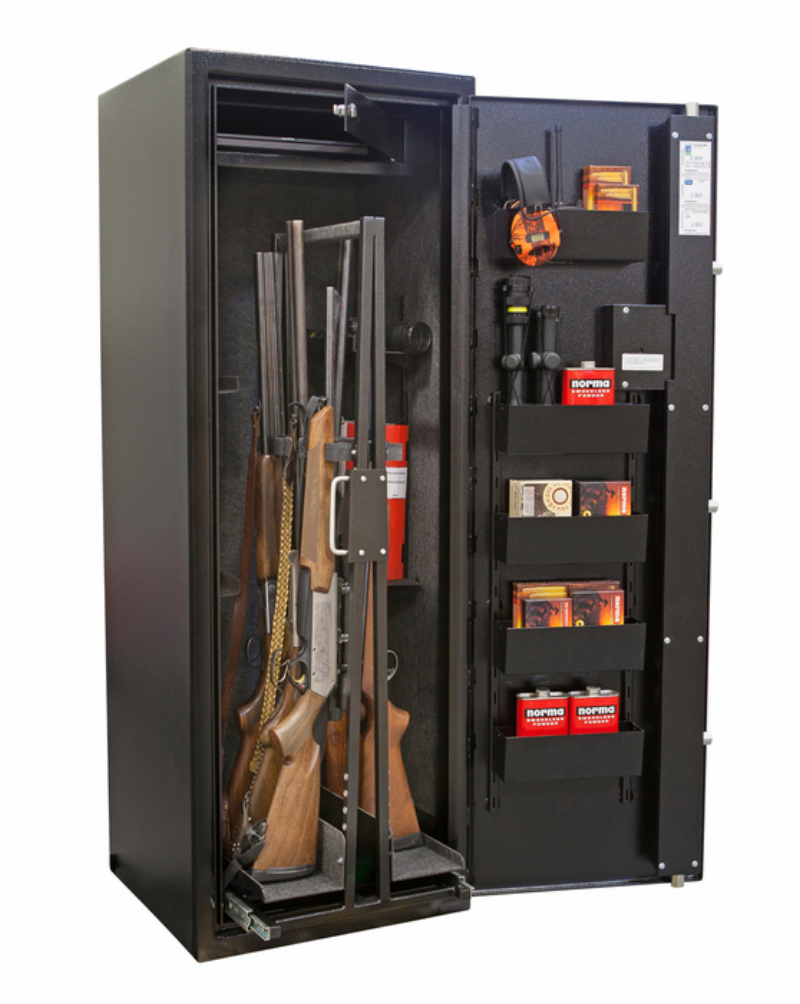
\includegraphics[width=0.8\linewidth]{Billeder/Redskaber/vaabenskab.png}



\end{columns}

\end{frame}